\chapter{Introduction}
\label{intro}

PrologPF is named after \textbf{Prolog} in \textbf{P}arallel with
\textbf{F}unctions.

PrologPF is an implementation of a parallel logic language with the
following key features:
\begin{itemize}
\item{The language is an extension of sequential Prolog \cite{CM87}.}
\item{Or-parallelism is provided through the use \textit{oracles} 
  (\cite{CA87} and section \ref{delphi_background}) to name branches
  in the search tree to be allocated for distributed search.}
\item{PrologPF extends the Prolog base language with
  support for the definition and deterministic
  application of higher-order functions
  in a manner consistent with the parallelisation method.}
\item{The target environment for the compiled binaries is a distributed
  network of heterogenous processors with comparatively slow communication
  links, such as an ethernet or wide-area internet.}
\item{The failure of individual processors during the parallel computation
  can be accomodated without undue performace penalty}
\end{itemize}

In comparison with other functional logic languages (Chapter \ref{background}),
PrologPF uses the
efficient but
incomplete depth-first search of standard Prolog and the deterministic
eager evaluation of function terms as in functional languages such as
Standard ML \cite{MTH90}.  PrologPF is a programming language for
\textit{realists} rather than 
a theorem proving system for \textit{purists} \cite{PS91}.

The primary goal the research described in this dissertation was to
exploit parallelism in a broader range of programs than was previously
possible using oracles, through the integration of functions into the
parallelised logic language.  PrologPF has been implemented and run with
a range of sample programs, such that that goal has been
achieved.

Considerable effort has been placed in maintaining the
portability of PrologPF.  The compiler
should provide a sound basis for further research such as:
\begin{itemize}
\item{Improvement of the strategies to
  be used for oracle distribution.}
\item{Extension of the oracles into
  the function evaluation trees.}
\end{itemize}

\subsection{Prolog}
%%%%%%%%%%%%

The definition of Standard Prolog is contained in \cite{DEC96}, and many
examples of practical use of the language in \cite{CM87}.

Prolog is a logic language based upon the first-order predicate calculus.\\
\todo{cite a predicate calculus ref}

A Prolog program
is a list of \textit{definite Horn clauses}, i.e. clauses containing exactly one
positive literal.  A clause with no positive literals defines the \textit{query}.
Each clause is a conjunction of literals.  A \textit{literal} is a predicate with
a list of terms as arguments.  A \textit{term} can be a \textit{constant} (i.e.
a string or number), a \textit{variable}, or a compound term. 
Variables are string constants beginning with a capital letter or \texttt{\_{}}.
A \textit{compound term}
is a string constant with a list of terms as arguments.

A clause containing one literal (which is positive) is called a \textit{fact}.  Clauses
with more than one literal (of which one is positive) are called \textit{rules}.

Prolog syntax requires that the positive literal appears at the head of the clause,
while the negative literals (called the \textit{body}
follow after the symbol \texttt{:-}.  The conjunction of
the negative literals is represented by \texttt{,}.  Clauses end with a full-stop (period).

Comments are surrounded by \texttt{/*\ldots*/} or by \texttt{\%\ldots<newline>}.

Examples of Prolog facts are:
\begin{verbatim}
a.              % the proposition a
a(b).           % relation a holds for term b
b(c).           % relation b holds for term c
a(b,c).         % relation a holds with arguments (b,c)
a(X).           % relation a holds for any argument term X
\end{verbatim}

Examples of Prolog rules are:
\begin{verbatim}
a :- b.         % asserts a & not(b), i.e. a <= b
a :- b,c.       % a & not(b) & not(c), i.e. a <= b & c
a(X) :- b(X).   % relation a holds for term X if relation b holds for same term
\end{verbatim}

\textit{Unification} is the process of matching a subgoal to the head of a clause,\\
\todo{unification reference}
arriving at a \textit{most general unifier} when the unification was successful.  The
unifier represents a set of variable bindings which would make the subgoal and the
head of the candidate clause identical.  These bindings form a context in which the
proof process continues.

In solving a query such as \texttt{:- a(X,Y),b(Y)} a sequential Prolog interpreter
will proceed from left-to-right, finding a solution for each subgoal in turn.  To
find a solution for a given subgoal (i.e. \texttt{a(X,Y)} first), the interpreter will
try the program clauses in a top-down order.  After a successful unification with the
head of a rule, the interpreter will attempt to solve left-to-right
the new goal defined by the
instantiated body of that rule.  On failure of this new subgoal, the top-down
search through the program clauses will continue.

\subsection{Parallelism}
%%%%%%%%%%%%

Logic languages have potential for faster execution through the
exploitation of the available parallelism \cite{Tic91}.  The 
declarative code can be parallelised in several ways, illustrated by the
following program fragment:

\begin{tabular}{l l l}
$a(X)$   &$\Leftarrow$ &$b(X,Y)\  \&\  b(Y,Y)$\\
$b(1,2)$ &             &\\
$b(2,2)$ &             &\\
\end{tabular}

A query can be expressed such as $a(Z)$
with the intended meaning that the system should
step through the program facts and rules to arrive at values for $Z$
for which $a(Z)$ is provable.

The opportunities for parallel execution
within the proof search process include:
\begin{description}
\item[And-parallelism]{The subgoals $b(X,Y)$ and $b(Y,Y)$
  in the body of the rule for $a$ may be searched in
  parallel to arrive at common solutions for $Y$}
\item[Or-parallelism]{The multiple rules for $b$ can be searched in
  parallel to find solutions for $b(X,Y)$ or $b(Y,Y)$.}
\item[Unification parallelism]{The subgoal $b(X,Y)$ can be solved if
  suitable values are found for both $X$ and $Y$.  In the selection of
  a candidate rule, these arguments can be unified in parallel with the
  formal arguments in the selected rule (e.g. ($1,2$))}
\end{description}

PrologPF implements or-parallelism through the use of \textit{oracles}
on an extended abstract machine called the \textit{Delphi machine}.
Further introduction is given in section \ref{delphi_background}, a
review of previous work on the Delphi machine in Chapter \ref{background},
and a detailed analysis of the technique in Chapter \ref{bfp_depth}.

\subsection{Functions}
%%%%%%%%%%%%

A detailed analysis of the functional support provided in PrologPF is
given in Chapter \ref{functions}.

Functional \textit{reduction} refers to the transformation of a reducible
term to a form which is irreducible.  When this process is
embedded in the code produced by compilation of a functional program, the
reduction is called \textit{evaluation}.

The execution of Prolog programs is limited to top-down, left-to-right
search with candidate clause matching through unification.  The
terms given as actual arguments to relations as subgoals are unified 
directly with the corresponding terms given as formal arguments in the
head of the candidate program clause.  Thus the Prolog system provides no
direct
support for the \textit{evaluation} of parameters (with the sole exception
of the \texttt{is} relation, see Chapter \ref{functions}).

However, equivalent relations can be defined representing the required
functions in a \textit{flat} form, with the result given as an
auxiliary argument.  For example the \texttt{length} function to
produce the length of a list can
be defined in Prolog as:
\begin{verbatim}
length([],0).
length([X|Y],N) :- length(Y,N1), N is N1 + 1.
\end{verbatim}

The \texttt{length} example illustrates the use of an auxiliary argument to
hold the result, and the flat form imposed by the exclusive use of 
relations, with the exception of the special \textit{is} which evaluates the
arithmetic expression given as the second argument.  With the definition
given above, the relation \texttt{length} can be used in a subgoal to
produce a variable binding for the length of a given list.  The Prolog
definition should be viewed in the context of these comments from
Compiling with Continuations, by Appel \cite{App92}:\\
\textit{The beauty of FORTRAN -- and the reason it was an improvement over
assembly language -- is that it relieves the programmer of the
obligation to make up names for intermediate results.  For example we write
$x = (a + b) * (c + d)$ instead of the assembly language:\\
\centerline{$r_1 \leftarrow a + b$}\\
\centerline{$r_2 \leftarrow c + d$}\\
\centerline{$x \leftarrow r_1 \times r_2$}\\
}

For comparison, a definition of \texttt{length} as a function in PrologPF
would be:
\begin{verbatim}
fun length([])    = 0;
    length([X|Y]) = 1 + length(Y).
\end{verbatim}

With the functional definition in PrologPF, the term \texttt{length(X)} can appear
anywhere in an argument term to represent the length of the list argument
\texttt{X}.

The reduction of functional expressions can be defined in terms of the
\textit{lambda calculus}\\
\todo{lambda calculus reference}
In lambda notation, terms are limited to:
\begin{description}
\item[Variables.]{Usually denoted by a constant string such as $x$.}
\item[Constants.]{Also denoted by constant strings, leaving context to
  differentiate constants and variables.}
\item[Applications.]{I.e. the application of a function $s$ to an
  argument $t$; both $s$ and $t$ may be arbitrary lambda terms.  An application
  can be represented by the simple juxstaposition of the function and argument,
  e.g. $s\ t$.  Application is generally defined to be left-associative, i.e.
  $s\ t\ u \equiv (s\ t)\ u$}
\item[Abstractions.]{I.e. function definitions in the lambda notation, the function
  mapping an argument $x$ to a term $t$ being $\lambda x.\ t$}
\end{description}

The application of an abstraction to an argument term relies upon the
principle of \textit{substitution}.  For example in the term
$(\lambda x.\ t)\ a$ the reduction of the application term proceeds with
the substitution of the argument $a$ for the variable $x$ in the term $t$, the
result denoted $t[a/x]$.  For example, $(\lambda x.\ x\ x)\ a$ reduces to
$(x\ x)[a/x]$, i.e. $(a\ a)$.

The $x$ in the above example is referred to as a \textit{bound} variable, representing
the formal argument of the lambda abstraction with the extent of its scope limited to
the abstraction body.  Terms within nested lambda abstractions may contain variables
other than those of the immediately enveloping lambda-term, and these variables are
said to be \textit{free} within that abstraction.  For example, in
$\lambda x.( \lambda y.\ x\ y)$ the variable $x$ is said to be free in the term
$\lambda y.\ x\ y$.  The set of free variables in a term $s$ can be denoted $FV(s)$, and 
the bound variables $BV(s)$.

Reduction in the lambda calculus is based upon three transformations of lambda terms:
\begin{description}
\item[1. $\alpha$-conversion.]{The constant representing the name of the bound variable
  in a lambda abstraction can be consistently changed throughout that expression, to any
  value that is not a free variable in the expression.  I.e. $\lambda x. s \rightarrow_\alpha
  \lambda y.s[y/x]$ provided $y \not \in FV(s)$}
\item[2. $\beta$-conversion.]{The application of a lambda abstraction to an argument
  term is equivalent to the body of the abstraction with the argument term 
  substituted for the bound variable.  I.e. $(\lambda x.\ s)\ t \rightarrow_\beta
  s[t/x]$.}
\item[3. $\eta$-conversion.]{A lambda abstraction which applies a term to the bound
  variable is equivalent to that term,
  provided the bound variable is free in the term.  I.e. $\lambda x.\ s\ x \rightarrow s$
  provided $x \not \in FV(s)$.}
\end{description}

The evaluation of lambda terms is equivalent to the repeated application of 
$\alpha$-, $\beta$- and $\eta$-conversions until there is nothing more to be 
evaluated.  When no more reductions are possible except for $\alpha$-conversions
the term is said to be in \textit{normal form}, and is \textit{irreducible}.

Within this framework there is still considerable flexibility in the selection of
the conversion to be applied at each step, and the selection of the subexpression
(the \textit{redex}) within the lambda term to be reduced.  For example, given:\\
\centerline{$(\lambda x.\ x\ x)\ ((\lambda y.\ a)\ a)$}\\
then an $\alpha$-conversion could be applied to either of the lambda-abstractions,
resulting in:\\
\centerline{$(\lambda y.\ y\ y)\ ((\lambda z.\ a)\ a)$}\\
or a $\beta$-conversion applied to the second application:\\
\centerline{$(\lambda x.\ x\ x)\ a$}\\
or a $\beta$-conversion applied to the first application:\\
\centerline{$((\lambda y.\ a)\ a)\ ((\lambda y.\ a)\ a))$}

Any implementation of a functional programming language based upon the lambda
calculus defines a \textit{reduction strategy}.  For the purposes of the
functional support in PrologPF the $\alpha$- and $\beta$-conversions are the
most significant, with the redex selection
for $\beta$-conversion being \textit{innermost first} for
nested lambda applications.

PrologPF provides a way of naming function abstractions (the \texttt{fun}
relation) and including lambda abstractions as argument terms (the 
\texttt{lambda} compound term).  Detail is given in Chapter \ref{functions}.

%%%%%%%%%%%%%%%%%%%%%%%%%%%%%%%%%%%%%%%%%%
\section{The Delphi Machine: Background} %
%%%%%%%%%%%%%%%%%%%%%%%%%%%%%%%%%%%%%%%%%%
\label{delphi_background}

This section provides an overview of or-parallel Prolog execution
using oracles.  A more detailed review of the prior work on the
Delphi machine is given in Chapter \ref{background}.

\subsection{The Delphi principle}
%%%%%%%%%%%%

The Delphi technique for or-parallel execution of logic programs
exploits the following:
\begin{enumerate}
\item{The search involved in the solution to a given query can
  be expressed as an \textit{or-only tree}.}
\item{Any point in the resultant search tree can be represented by
  a sequence of integers giving the path to be taken at each internal
  node leading from the root of the tree to the selected point.
  The sequence of integers is called an \textit{oracle}}
\item{The environment at a given point in the search can be
  recreated by following the associated oracle, and the search continued
  from there.}
\end{enumerate}

The technique can be illustrated by the following example:

\begin{figure}[h]
\vspace{5mm} \hbox to \hsize{\hfill \psfig{file={intro/ps/and_or_tree.ps}} \hfill}
\caption{Search tree for goal clause g(U,V).}
\vspace{5mm}
\label{and_or_tree}
\end{figure}

Figure \ref{and_or_tree} (from \cite{CA87}) shows the \textit{and-or tree} for
the Prolog program given on the left.

The and-or tree consists of nodes representing the conjunctive subgoals from
the body of the rule (i.e. the and-node from \texttt{g(U,V) :- p(U),q(V),r(U,V)}),
and or-nodes from the alternate clauses available for the solution of each
subgoal.  The \texttt{p(U)} subgoal transforms to an or-node with the two
children \texttt{p(1)} and \texttt{p(2)}.

The strict depth-first left-to-right execution strategy of Prolog ensures that
a solution to the subgoal \texttt{p(U)} is found before execution proceeds with
a search for a solution to \texttt{q(V)}, and then for \texttt{r(U,V)}.
This means that the subtree for \texttt{q(V)} can be moved and replicated under
each leaf-node of the subtree for \texttt{p(U)}
(figure \ref{or_only_tree} First Stage).
 The subtree for \texttt{r(U,V)}
can then be moved and replicated below each of the resultant leaf nodes, arriving
at the or-only tree in figure \ref{or_only_tree} (Second Stage).

\begin{figure}[htb]
\vspace{5mm} \hbox to \hsize{\hfill \psfig{file={intro/ps/or_only_tree.ps}} \hfill}
\caption{Transformation to an or-only tree.}
\vspace{5mm}
\label{or_only_tree}
\end{figure}

The or-parallelism exploited in PrologPF is equivalent to parallel search
of subtrees of the or-only tree in figure \ref{or_only_tree}.  If integers are
used to label each branch at each or-node (figure \ref{oracle_tree}) then the
sequence of integers leading to a subtree is an \textit{oracle}.

\begin{figure}[htb]
\vspace{5mm} \hbox to \hsize{\hfill \psfig{file={intro/ps/oracle_tree.ps}} \hfill}
\caption{Or-only tree with integer branch labels.}
\vspace{5mm}
\label{oracle_tree}
\end{figure}

In figure \ref{oracle_tree} each leaf node is labelled with the associated oracle,
and the two major subtrees in this example can be labelled with the oracles
$[1]$ and $[2]$ respectively.

An oracle forms a compact representation of any point within the Prolog
search tree for a program with a given query, and parallel computation of the
query can be implemented by passing oracles to distributed Delphi machines
(also called \textit{path processors}, Section \ref{path_processors})
with an associated \textit{strategy} (Section \ref{delphi_strategies}).

If each \textit{n}-branch node in the or-only tree is replaced by a
number of binary nodes through the insertion of dummy nodes, then the
or-only tree becomes a \textit{binary or-only tree} with the characteristic
that the oracles become binary strings, rather than sequences of natural numbers.
This may benefit the generation of oracles using strategies not involving
partial search of the proof tree.  The strategies used in PrologPF (Chapter
\ref{bfp_depth}) all use partial search to generate oracles, such that
the \textit{n}-ary tree representation is sufficient to describe the
operational semantics.
 
\subsection{Path processors}
%%%%%%%%%%%%
\label{path_processors}

The distributed \textit{path processors} provide the support for the execution of
the logic program, with the abstract machine extended to generate and
follow oracles.  To accomodate a wide range of distributed execution
strategies (Section \ref{delphi_strategies}), the oracle support can
include the following:

\begin{enumerate}
\item{Given an oracle, the path processor can follow that oracle from the
  root of the search tree and report the status of that oracle:
  \begin{description}
  \item[Fail:]{The oracle resulted in  \textit{failure}, either at the end or along 
    its path}
  \item[Success:]{During execution of the oracle, a solution was found.
    This may occur with a prefix of the oracle, or may have
    used every integer in the oracle string.  The path processor can
    report the solution with the oracle defining its position in the
    proof tree.}
  \item[Open:]{The last or-choice indicated by the last integer of the
    oracle lead to a successful unification with the head of a rule, such
    that the execution of the oracle has led to neither \textit{success}
    or \textit{fail}.}
  \end{description}}
\item{The path processor can be asked to search the proof tree within some
  bound (for example a fixed depth), and to report the open oracles found
  within that bound.}
\item{The path processor may be interrupted, when it should pause and report
  the oracle representing its current search position.}
\end{enumerate}

The implementation of the Delphi machine embedded within PrologPF combines the
capabilities described in 1 and 2 above, such that the path processor represented
by the executing compiled program can:
\begin{enumerate}
\item{accept a depth bound $L$ as a control parameter which can be zero, any
  positive integer, or a special value representing infinity}
\item{follow a given oracle to its end, reporting \textit{success} or
  \textit{failure} if that occurs}
\item{continue searching from the end of the given oracle to an incremental
  depth $L$, reporting any solutions found within that depth and generating
  and reporting the open oracles at that depth bound.}
\end{enumerate}

When one PrologPF binary partially searches the proof tree to generate
an oracle (or many) for distribution to other processors to follow,
the distributed system involves a significant amount 
of \textit{recomputation}.
The Delphi approach trades off the overhead of recomputation with the minimal
communications requirement of most successful distributed execution
strategies.

\subsection{Delphi strategies}
%%%%%%%%%%%%
\label{delphi_strategies}

The binary produced by the PrologPF compiler will execute sequentially on
any suitable workstation.  Speedup though distributed processing is
achieved though the coordinated execution of the same binary on a network
of similar workstations used as path processors, with a separate
workstation (the \textit{control processor}) controlling the work flow.

The control processor can define the \textit{strategy} to be used for
the allocation of work.

As a simple (and very inefficient) example, the control processor could
generate oracles at random.  These could be sent to randomly selected
path processors (with an incremental depth bound $L$ of 0, see Section
\ref{path_processors}) until a solution were found.

The support for oracles embedded within PrologPF binaries is sufficient to
implement a wide range of strategies.  The strategies evaulated in this and
previous research include (see Chapter \ref{background}):

\begin{itemize}
\item{\textbf{Non-backtracking strategies:}
  \begin{description}
    \item[\textit{Brute Force}:]{ \cite{CA87}.
       The random allocation of oracles described above}
    \item[\textit{Branch-by-branch}:]{ \cite{Kle91}. 
      The depth bound $L$ is fixed at 1, and
      starting at the root of the proof tree, the oracle is extended one digit at
      a time.  I.e. a path processor reports the open single-digit oracles from
      the root, which are redistributed to the path processors, which report back the
      open two-digit oracles and so on.}
    \item[\textit{Expanding a Job}:]{ \cite{CA87}.
      As with \textit{branch-by-branch}, except
      the proof tree is treated as a binary tree, and the oracle is extended a
      \textit{bit} at a time.}
  \end{description}}
\item{\textbf{Backtracking strategies:}
  \begin{description}
    \item[\textit{Automatic Partitioning}:]{ \cite{Kle91}.
      Each path processor is given $G$, the number of path processors in the pool,
      and $N$ the individual processor number.  Each path processor uses these numbers to
      arrive at a unique subtree within the proof tree.  At each choice point a
      given path processor can select a path modulo $G$ with offset $N$ (see 
      Chapter \ref{background} for further detail) and can identify the point at which
      the path becomes unique to that path processor.  The path processor then
      searches the subtree below this point without constraint.}
    \item[\textit{Reassign-Job}:]{ \cite{Kle91}.
      This is a modification to \textit{Automatic Partitioning} to allow path
      processors encountering \textit{failure} to register with the control
      processor for further work.  Busy path processors are required to poll
      the control processor (in the Klein implementation) to communicate their
      current oracle for re-partitioning.}
    \item[\textit{Breadth-first Partitioning}:]{ \cite{Sar95} and Chapter \ref{bfp_depth}.
      An initial run takes place with a depth bound $L$ set to generate a
      suitable number of oracles.  These oracles are then all allocated among
      the available path processors.  The path processors follow each assigned
      oracle, and fully search the subtree below each.}
    \item[\textit{Partitioning by Selective Sampling}:]{ \cite{Sar95}.
      This strategy attempts to improve the effectiveness of the
      one-time allocation of oracles
      to path processors by estimating the work beneath each oracle generated in
      the depth-constrained first phase of breadth-first partitioning.  These
      estimates are used to achieve a more balanced allocation of the oracles
      to the path processors for subsequent unconstrained search.  The work beneath
      each oracle is estimated by partially searching the subtree (with a limit
      set on the number of choice-points traversed) and accumulating the
      number of or-branches passed during the search.}
    \item[\textit{Breadth-first Partitioning with Selective Sampling}:]{ \cite{Sar95}.
      The final strategy from Saraswat's research has the same goal of improving
      the allocation of the oracles from an initial breadth-first phase.  The
      method used in this strategy is to fully search the subtree below every other
      oracle, and use the arithmetic mean of the nodes encountered as a measure of
      the work associated with the intermediate oracles.}
  \end{description}}
\end{itemize}


%%%%%%%%%%%%%%%%%%%%%%%%%%%%%%%%%%%%%%%%%%%%%%%
\section{The Delphi Machine and \textit{cut}} %
%%%%%%%%%%%%%%%%%%%%%%%%%%%%%%%%%%%%%%%%%%%%%%%

\todo{include Italian cut reference}

This section gives an overview of the issues surrounding the metalogical \textit{cut}
relation (written '\texttt{!}' in Prolog).  The topic is covered in detail in
Chapter \ref{cut}.

Figure \ref{cut_tree} shows the clauses and associated or-only tree for a 
program containing \textit{cut}.  The procedure for \texttt{r} is intended as
a function that maps a first argument
 \texttt{1} to \texttt{10}, and any other first argument
to \texttt{2}:
\begin{verbatim}
r(1,10) :- !.
r(X,2).
\end{verbatim}

A sequential implementation of Prolog will prune away
the solution from the second clause
for \texttt{r(1,X)}.  Without the \textit{cut}, there would be two solutions, i.e.
\texttt{\{X = 10, X = 2\}}.
  In an or-parallel system such as PrologPF, the cut must be
communicated at run-time
across processor boundaries (represented by the dashed-arrows in
figure \ref{cut_tree}).

In systems implementing the Delphi principle, communication down
a path in the tree can be considered to be inexpensive, while between branches
(i.e. possibly between path processors) communication may be expensive.

\begin{figure}[h]
\vspace{5mm} \hbox to \hsize{\hfill \psfig{file={intro/ps/cut_tree.tgif.eps}} \hfill}
\caption{Prolog implementation of r(U,V) with cut and transformed tree.}
\vspace{5mm}
\label{cut_tree}
\end{figure}

In PrologPF, alternative or-paths in the proof tree may be executed asynchronously, such
that the recognition of the cut is likely to occur after the tree has split further, and
communication will be needed between multiple path processors.

A general support for \textit{cut} within the or-parallel framework of distributed
Delphi machines would require a communications system to propagate the \textit{cut} to
those path processors searching subtrees that should be pruned.
The pruning operation may in effect be a truncation
of an allocated oracle,
or it may affect the subtree beneath an oracle.  Oracle management is thus more complicated.
However, the two most critical issues affecting the implementation of general \textit{cut}
support within PrologPF are:
\begin{enumerate}
\item{The \textit{cut} within the program can be expected to be executed many times,
  generating a great deal of communications traffic if a general distributed support were
  implemented.  PrologPF succeeds in a network of general purpose workstations because
  the communications traffic is kept to a minimum.}
\item{The delivery of solutions to a client would have to be delayed until all the
  path processors have completed, to ensure that all solutions below any \textit{cut}
  are correctly pruned.  A major strength of PrologPF is the efficient delivery
  of a first solution.}
\end{enumerate}


%%%%%%%%%%%%%%%%%%%%%%%%%%%%%%%%%%%%%%%%%%%%
\section{The Delphi Machine and functions} %
%%%%%%%%%%%%%%%%%%%%%%%%%%%%%%%%%%%%%%%%%%%%

For a detailed discussion of the functional support in PrologPF see
Chapter \ref{functions}.

The support for \textit{cut} in PrologPF recognises that a major requirement for the
metalogical predicate is to enforce determinism in user code.
Deterministic code does not contain any choice points, and the presence of the 
\textit{cut} thus does not conflict with the or-parallelism implemented in
PrologPF.  An example illustrating this is given later in this section.

While \textit{cut} can be used to enforce determinism, \textit{cut} can also be
used in nondeterministic relations (those returning multiple solutions).  Also
a relation containing \textit{cut} may be deterministic with one set of actual
arguments, but nondeterministic with another.

The implementation of or-parallelism using the Delphi machine in PrologPF requires that
determinism is explicit through the use of \textit{functions} rather than
relations containing \textit{cut}.  The evaluation of functions in PrologPF
is defined to be deterministic.  As oracles add no information when the execution tree
is linear
(i.e. representing a deterministic execution), oracle support can be switched off
(see below) while functional evaluation occurs.

The example in figure \ref{fun_tree3} shows a program similar to that using cuts given
earlier in figure \ref{cut_tree}, but instead uses a function to define \texttt{r}.
As progression down the tree represents the execution of the program, the function
evaluation can be represented as the linear subtree embedded on the right of the
proof tree.

\begin{figure}[h]
\vspace{5mm} \hbox to \hsize{\hfill \psfig{file={intro/ps/fun_tree3.tgif.eps}} \hfill}
\caption{Program and search tree for program with function r(X).}
\vspace{5mm}
\label{fun_tree3}
\end{figure}

Figure \ref{fun_tree4} shows the transformation of the search tree into an
or-only tree suitable for labelling with oracles for allocation to
distributed Delphi machines.  The linear portions due to the functional evaluation
can be seen, and it is clear that the integer labels of the or-branches can
be limited to the alternatives for \texttt{p(U)} and \texttt{q(\_{}V)}. The path
defined by the oracle can be imagined to jump from the last or-choice to the
end of the functional evaluation, and continue from there.

\begin{figure}[h]
\vspace{5mm} \hbox to \hsize{\hfill \psfig{file={intro/ps/fun_tree4.tgif.eps}} \hfill}
\caption{Transformation of tree containing r(X) to or-only tree.}
\vspace{5mm}
\label{fun_tree4}
\end{figure}

The deterministic evaluation of functions is crucial to the 
technique of partial suspension of
oracle processing used in PrologPF.  This ensures that the oracle leading to the 
start of the functional evaluation branch can equally be said to lead to the 
branching point of the next or-choice.

Other functional logic languages (See Chapter \ref{background}) aim for
completeness in the combined paradigms, providing non-deterministic
reduction of functions.  The deterministic evaluation of functions in PrologPF
was chosen for compatibility with the efficient implementation on the
Delphi machine, compensating for the removal of \textit{cut}.

%%%%%%%%%%%%%%%%%%%%%%%%%%%%%%%
\section{Research Motivation} %
%%%%%%%%%%%%%%%%%%%%%%%%%%%%%%%

Prior work on implemenations of Prolog with the Delphi principle
\cite{Kle91, Sar95} have shown the suitability of the method for
or-parallel execution of pure Prolog programs in distributed systems
with relatively high communications costs.

The computing trends exploited by the technique can be expected to
continue:
\begin{enumerate}
\item{The processor performance of generally available computers
  is increasing faster than the performance of generally available
  network connections.}
\item{The number of general-purpose processors available within
  a general network environment (i.e. Ethernet or the internet)
  is increasing.}
\end{enumerate}

Given the success of the technique with pure Prolog programs
\cite{Sar95}, a compatible extension to Prolog to allow the use
of functions should bring the benefits of parallel execution
with the Delphi principle to
a broader range of problems.

%%%%%%%%%%%%%%%%%%%%%%%%%%
\section{Research Goals} %
%%%%%%%%%%%%%%%%%%%%%%%%%%

\begin{itemize}
\item{to gain further insight into the behaviour patterns of
  existing execution algorithms exploiting the Delphi principle}
\item{to extend the Prolog on the Delphi machine with functional features
  mitigating the removal of \textit{cut}}
\item{to implement a general purpose control system suitable for
  managing the distributed execution of the path processors}
\item{to test the combined system with a much broader range of
  Prolog and other code than has been attempted previously}
\end{itemize}

%%%%%%%%%%%%%%%%%%%%%%%%%
\section{Contributions} %
%%%%%%%%%%%%%%%%%%%%%%%%%

The research documented in this dissertation shows that the Prolog
language can be extended with higher-order functions in a manner
consistent with the or-parallel execution of a program with oracles.
The combined language can be effectively
applied to a broader range of problems than was possible with pure
Prolog on previous implementations of the Delphi machine.

The PrologPF 
implementation is sufficient to study a range of oracle assignment
strategies, and the influence of the depth parameter $L$ on the
breadth-first partitioning strategy was studied in detail.

%%%%%%%%%%%%%%%%%%%%%%%%%%%%%%%%
\section{Dissertation Outline} %
%%%%%%%%%%%%%%%%%%%%%%%%%%%%%%%%

\todo{describe toc}
